\documentclass{standalone}
\usepackage{tikz}
\usetikzlibrary{patterns, positioning}

\begin{document}
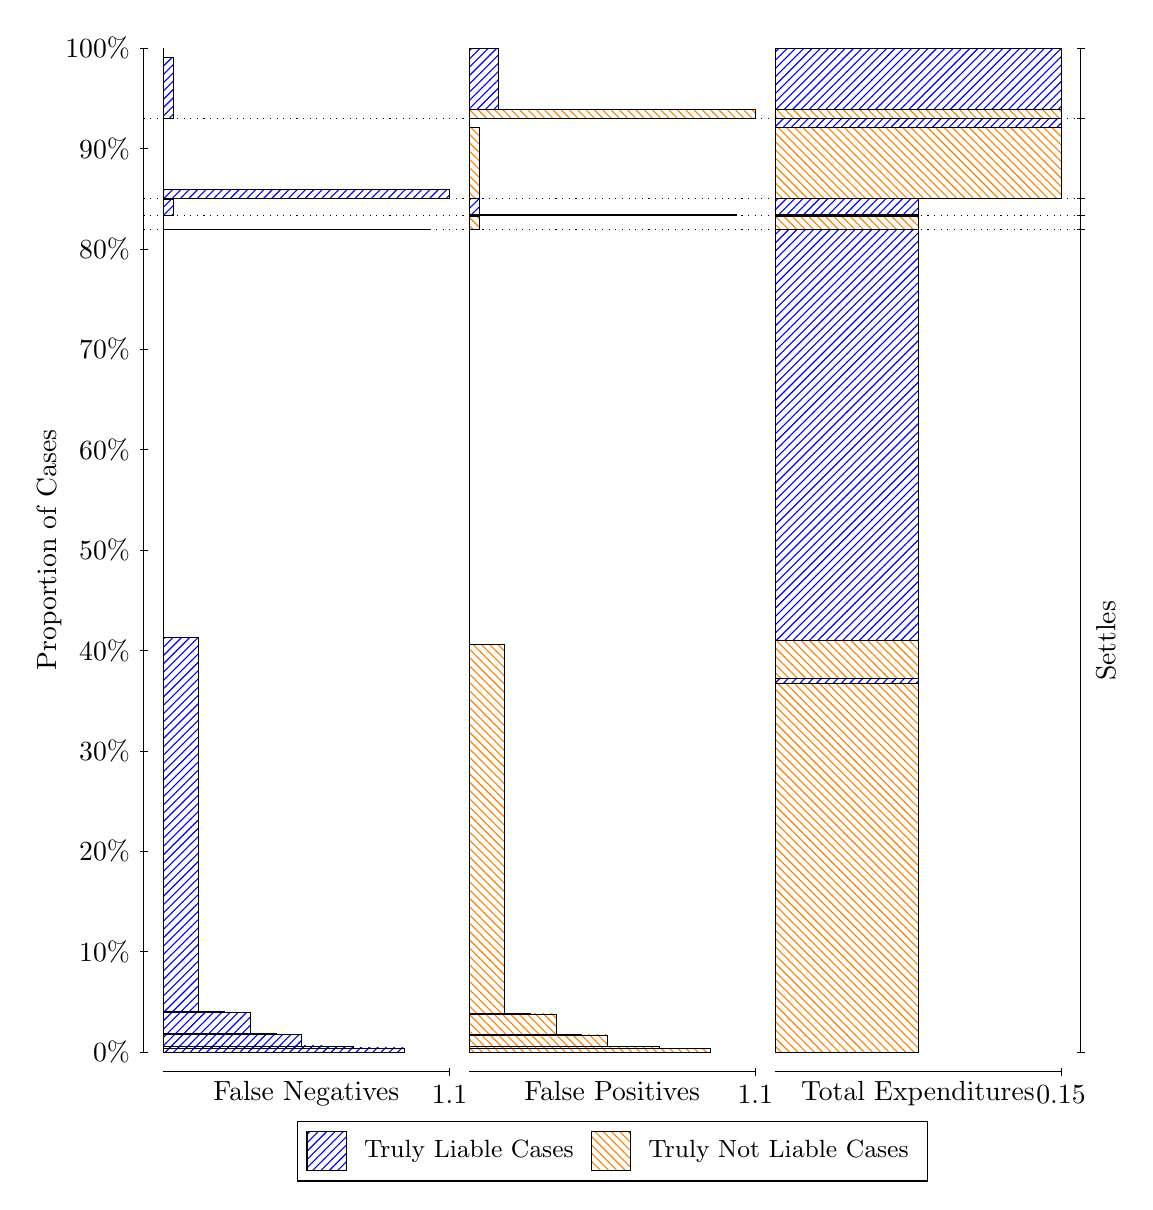
\begin{tikzpicture}
\draw[black, very thin] (1.5,1.75) -- (1.5,14.5);
\node[rotate=90, anchor=center] at (0.3, 8.125) {Proportion of Cases};
\draw[black, very thin] (1.45,1.75) -- (1.55,1.75);
\node[anchor=east] at (1.45, 1.75) {0\%};
\draw[black, very thin] (1.45,3.025) -- (1.55,3.025);
\node[anchor=east] at (1.45, 3.025) {10\%};
\draw[black, very thin] (1.45,4.3) -- (1.55,4.3);
\node[anchor=east] at (1.45, 4.3) {20\%};
\draw[black, very thin] (1.45,5.575) -- (1.55,5.575);
\node[anchor=east] at (1.45, 5.575) {30\%};
\draw[black, very thin] (1.45,6.85) -- (1.55,6.85);
\node[anchor=east] at (1.45, 6.85) {40\%};
\draw[black, very thin] (1.45,8.125) -- (1.55,8.125);
\node[anchor=east] at (1.45, 8.125) {50\%};
\draw[black, very thin] (1.45,9.4) -- (1.55,9.4);
\node[anchor=east] at (1.45, 9.4) {60\%};
\draw[black, very thin] (1.45,10.675) -- (1.55,10.675);
\node[anchor=east] at (1.45, 10.675) {70\%};
\draw[black, very thin] (1.45,11.95) -- (1.55,11.95);
\node[anchor=east] at (1.45, 11.95) {80\%};
\draw[black, very thin] (1.45,13.225) -- (1.55,13.225);
\node[anchor=east] at (1.45, 13.225) {90\%};
\draw[black, very thin] (1.45,14.5) -- (1.55,14.5);
\node[anchor=east] at (1.45, 14.5) {100\%};

\draw[black, very thin] (13.4,1.75) -- (13.4,14.5);
\draw[black, very thin] (13.35,1.75) -- (13.45,1.75);
\node[anchor=west] at (13.35, 1.75) {};
\draw[black, very thin] (13.35,12.192) -- (13.45,12.192);
\node[anchor=west] at (13.35, 12.192) {};
\draw[black, very thin] (13.35,12.37) -- (13.45,12.37);
\node[anchor=west] at (13.35, 12.37) {};
\draw[black, very thin] (13.35,12.592) -- (13.45,12.592);
\node[anchor=west] at (13.35, 12.592) {};
\draw[black, very thin] (13.35,13.605) -- (13.45,13.605);
\node[anchor=west] at (13.35, 13.605) {};
\draw[black, very thin] (13.35,14.5) -- (13.45,14.5);
\node[anchor=west] at (13.35, 14.5) {};

\draw[black, very thin, pattern color=blue, pattern=north east lines] (1.75,1.75) rectangle (4.8118,1.8014);
\draw[black, very thin, pattern color=blue, pattern=north east lines] (1.75,1.8014) rectangle (4.4852,1.803);
\draw[black, very thin, pattern color=blue, pattern=north east lines] (1.75,1.803) rectangle (4.1586,1.8245);
\draw[black, very thin, pattern color=blue, pattern=north east lines] (1.75,1.8245) rectangle (3.832,1.8267);
\draw[black, very thin, pattern color=blue, pattern=north east lines] (1.75,1.8267) rectangle (3.5054,1.978);
\draw[black, very thin, pattern color=blue, pattern=north east lines] (1.75,1.978) rectangle (3.1788,1.9858);
\draw[black, very thin, pattern color=blue, pattern=north east lines] (1.75,1.9858) rectangle (2.8522,2.2577);
\draw[black, very thin, pattern color=blue, pattern=north east lines] (1.75,2.2577) rectangle (2.5257,2.262);
\draw[black, very thin, pattern color=blue, pattern=north east lines] (1.75,2.262) rectangle (2.1991,7.0194);
\draw[black, very thin, pattern color=orange, pattern=north west lines] (1.75,7.0194) rectangle (1.75,12.192);
\draw[black, very thin, pattern color=blue, pattern=north east lines] (1.75,12.192) rectangle (5.1384,12.201);
\draw[black, very thin, pattern color=orange, pattern=north west lines] (1.75,12.201) rectangle (1.75,12.37);
\draw[black, very thin, pattern color=blue, pattern=north east lines] (1.75,12.37) rectangle (1.8725,12.578);
\draw[black, very thin, pattern color=orange, pattern=north west lines] (1.75,12.578) rectangle (1.75,12.592);
\draw[black, very thin, pattern color=blue, pattern=north east lines] (1.75,12.592) rectangle (5.3833,12.705);
\draw[black, very thin, pattern color=orange, pattern=north west lines] (1.75,12.705) rectangle (1.75,13.605);
\draw[black, very thin, pattern color=blue, pattern=north east lines] (1.75,13.605) rectangle (1.8725,14.38);
\draw[black, very thin, pattern color=orange, pattern=north west lines] (1.75,14.38) rectangle (1.75,14.5);
\draw[black, very thin, pattern color=orange, pattern=north west lines] (5.6333,1.75) rectangle (8.6951,1.7977);
\draw[black, very thin, pattern color=orange, pattern=north west lines] (5.6333,1.7977) rectangle (8.3685,1.7991);
\draw[black, very thin, pattern color=orange, pattern=north west lines] (5.6333,1.7991) rectangle (8.0419,1.8203);
\draw[black, very thin, pattern color=orange, pattern=north west lines] (5.6333,1.8203) rectangle (7.7154,1.8226);
\draw[black, very thin, pattern color=orange, pattern=north west lines] (5.6333,1.8226) rectangle (7.3888,1.9676);
\draw[black, very thin, pattern color=orange, pattern=north west lines] (5.6333,1.9676) rectangle (7.0622,1.971);
\draw[black, very thin, pattern color=orange, pattern=north west lines] (5.6333,1.971) rectangle (7.0622,1.9772);
\draw[black, very thin, pattern color=orange, pattern=north west lines] (5.6333,1.9772) rectangle (6.7356,2.2351);
\draw[black, very thin, pattern color=orange, pattern=north west lines] (5.6333,2.2351) rectangle (6.409,2.2415);
\draw[black, very thin, pattern color=orange, pattern=north west lines] (5.6333,2.2415) rectangle (6.0824,6.9226);
\draw[black, very thin, pattern color=blue, pattern=north east lines] (5.6333,6.9226) rectangle (5.6333,12.192);
\draw[black, very thin, pattern color=orange, pattern=north west lines] (5.6333,12.192) rectangle (5.7558,12.361);
\draw[black, very thin, pattern color=blue, pattern=north east lines] (5.6333,12.361) rectangle (5.6333,12.37);
\draw[black, very thin, pattern color=orange, pattern=north west lines] (5.6333,12.37) rectangle (9.0217,12.384);
\draw[black, very thin, pattern color=blue, pattern=north east lines] (5.6333,12.384) rectangle (5.7558,12.592);
\draw[black, very thin, pattern color=orange, pattern=north west lines] (5.6333,12.592) rectangle (5.7558,13.492);
\draw[black, very thin, pattern color=blue, pattern=north east lines] (5.6333,13.492) rectangle (5.6333,13.605);
\draw[black, very thin, pattern color=orange, pattern=north west lines] (5.6333,13.605) rectangle (9.2667,13.725);
\draw[black, very thin, pattern color=blue, pattern=north east lines] (5.6333,13.725) rectangle (6.0007,14.5);
\draw[black, very thin, pattern color=orange, pattern=north west lines] (9.5167,1.75) rectangle (11.333,6.4375);
\draw[black, very thin, pattern color=blue, pattern=north east lines] (9.5167,6.4375) rectangle (11.333,6.4905);
\draw[black, very thin, pattern color=orange, pattern=north west lines] (9.5167,6.4905) rectangle (11.333,6.9757);
\draw[black, very thin, pattern color=blue, pattern=north east lines] (9.5167,6.9757) rectangle (11.333,12.192);
\draw[black, very thin, pattern color=orange, pattern=north west lines] (9.5167,12.192) rectangle (11.333,12.361);
\draw[black, very thin, pattern color=blue, pattern=north east lines] (9.5167,12.361) rectangle (11.333,12.37);
\draw[black, very thin, pattern color=orange, pattern=north west lines] (9.5167,12.37) rectangle (11.333,12.384);
\draw[black, very thin, pattern color=blue, pattern=north east lines] (9.5167,12.384) rectangle (11.333,12.592);
\draw[black, very thin, pattern color=orange, pattern=north west lines] (9.5167,12.592) rectangle (13.15,13.492);
\draw[black, very thin, pattern color=blue, pattern=north east lines] (9.5167,13.492) rectangle (13.15,13.605);
\draw[black, very thin, pattern color=orange, pattern=north west lines] (9.5167,13.605) rectangle (13.15,13.725);
\draw[black, very thin, pattern color=blue, pattern=north east lines] (9.5167,13.725) rectangle (13.15,14.5);
\draw[black, dotted] (1.5,12.192) -- (13.4,12.192);
\draw[black, dotted] (1.5,12.37) -- (13.4,12.37);
\draw[black, dotted] (1.5,12.592) -- (13.4,12.592);
\draw[black, dotted] (1.5,13.605) -- (13.4,13.605);
\draw[black, very thin] (1.75,1.5) -- (5.3833,1.5);
\node[anchor=north] at (3.5667, 1.5) {False Negatives};
\draw[black, very thin] (5.3833,1.45) -- (5.3833,1.55);
\node[anchor=north] at (5.3833, 1.45) {1.1};

\draw[black, very thin] (5.6333,1.5) -- (9.2667,1.5);
\node[anchor=north] at (7.45, 1.5) {False Positives};
\draw[black, very thin] (9.2667,1.45) -- (9.2667,1.55);
\node[anchor=north] at (9.2667, 1.45) {1.1};

\draw[black, very thin] (9.5167,1.5) -- (13.15,1.5);
\node[anchor=north] at (11.333, 1.5) {Total Expenditures};
\draw[black, very thin] (13.15,1.45) -- (13.15,1.55);
\node[anchor=north] at (13.15, 1.45) {0.15};

\node[black, centered, rotate=90] at (13.72, 6.971) {Settles};





\draw (7.449999999999999,1.5) node[draw=none] (baseCoordinate) {};
\begin{scope}[align=center]
        \matrix[scale=0.5, draw=black, below=0.5cm of baseCoordinate, nodes={draw}, column sep=0.1cm]{
            \node[rectangle, draw, minimum width=0.5cm, minimum height=0.5cm, pattern=north east lines, pattern color=blue] {}; &
            \node[draw=none, font=\small] (B) {Truly Liable Cases}; &
            \node[rectangle, draw, minimum width=0.5cm, minimum height=0.5cm, pattern=north west lines, pattern color=orange] {}; &
            \node[draw=none, font=\small] (B) {Truly Not Liable Cases}; \\
            };
\end{scope}

\end{tikzpicture}
\end{document}